\chapter{Lights Out}

In this chapter I give a tour of the puzzle game \lo by Tiger Electronics.

\section{Description}

\begin{figure}[bh]
	\begin{center}
		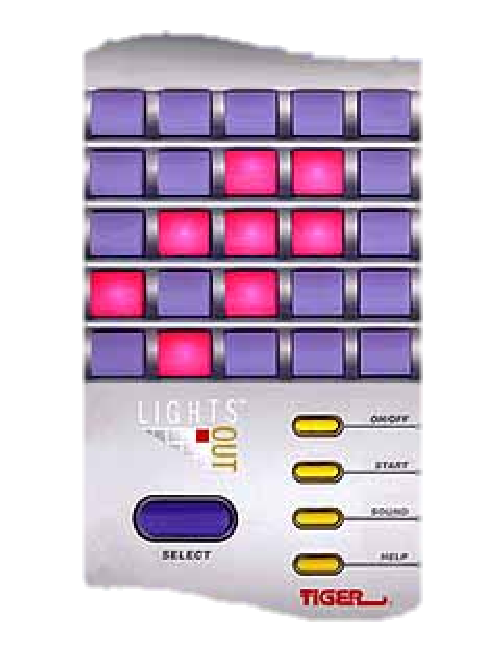
\includegraphics[width=\linewidth/3]{image/lightout.ps}
		\caption{Handheld puzzle game Lights Out}\label{figure:puzzle}
	\end{center}
\end{figure}
\lo is a handheld puzzle game produced by Tiger Toys\footnote{Tiger Toys is now
incorparated in Hasbro. Hasbro renamed it Tiger Electronics}. (See figure
\ref{figure:puzzle}) It consists of a five by five grid of buttons that double
as lights. Each button can be in two possible states: on (lit) and off (unlit).

The goal of the game is to change all buttons to the unlit state. This can be
achieved by pressing buttons. A button press has the effect of changing state on
itself and on the vertical and horizontal neighbouring buttons.

There are various modes on \lo. In one mode one has to solve predetermined
puzzles which gradually increase in difficulty. The random mode presents you
with a random configuration of lit buttons. There is also a mode where one can
invent ones own pattern of lit buttons. 

\section{Solving Lights Out}

Figure \ref{figure:pairs} lists all essentially different possible
configurations of a pressing pair of buttons. Essentialy different means that
pressing a pair of buttons can be brought to coincide with one of the five
configurations\footnote{Notice that one configuration is actually a class of
different configurations.} by translation, rotation or combinations of the two.
\begin{figure}
	\begin{center}
		\subfigure[$d>2$]{\includegraphics[width=25mm]{image/button_presses1.ps}}
		\hfill
		\subfigure[$d=2$]{\includegraphics[width=25mm]{image/button_presses3.ps}}
		\hfill
		\subfigure[$d=2$]{\includegraphics[width=25mm]{image/button_presses2.ps}}
		\hfill
		\subfigure[$d=1$]{\includegraphics[width=25mm]{image/button_presses4.ps}}
		\hfill
		\subfigure[$d=0$]{\includegraphics[width=25mm]{image/button_presses5.ps}}\label{figure:sub:zero}
	\end{center}
	\caption{The essential different possible positions of a pair of
	buttons.}\label{figure:pairs}
\end{figure}

The configurations are ordered by the distance $d$ between the two different
pressed buttons. (The distance used is the Manhattan distance.)

In the configurations in figure \ref{figure:pairs} a button has changed state
after pressing the pair of buttons if the button is lined. A button did
not change state if the button is hatched. Because the state of a button is
determined by the parity of the number of neighbours that get pressed, it is
clear that the order in which buttons get pressed is irrelevant.

Because the order in which the buttons are pressed is irrelevant we can choose
our favourite order. Our order will be: In every row from left to right and the
rows from top to bottom.

Figure \ref{figure:pairs} tells us something else. In the last configuration a
button is pressed twice. The effect is that all buttons change state twice. So
they do not change state at all. We now know that a button never has to be
pressed more than once.

Imagine that we are presented with a puzzle and we found a solution. Because the
order in which we press the buttons is row by row and in every row from left to
right we can deduce the following fact.
\begin{figure}
	\begin{center}
		\hspace*{\fill}
		\subfigure[Before]{\includegraphics[width=35mm]{image/chasing_lights1.ps}}
		\hfill
		\subfigure[After]{\includegraphics[width=35mm]{image/chasing_lights2.ps}}
		\hspace*{\fill}
	\end{center}
	\caption{Pressing buttons in the first row.}\label{figure:chasing}
\end{figure}

Say we have pressed all buttons in the first row and glance at the resulting
pattern of lit buttons. (See also figure \ref{figure:chasing} for an example.
There every button with a cross must be pressed.) Pretend that there are still
lit buttons in the first row. These buttons must change state, but the only
buttons that can influence these buttons are in the second row. In particular
every button in the second row influences exactly one button in the first row. A
button influences the button directly above itself.

So once the buttons in the first row are pressed, it is clear which buttons must
be pressed in the second row. These are the buttons directly under the lit
buttons of row 1. The same reasoning holds for the buttons in the third row. In
fact the reasoning holds all the way down to the last row. Lets call this
process \emph{chasing down the lights}.

So lets examine what happens if we press a button in the first row and
diligently chase the lights down. Table \ref{table:effects} summarizes the
effect chasing down each button in the first row.
The numbers in the first column (labelled ``Button'') refer to the buttons in
the first row. The numbers in the second row (underneath the row labelled
``Effect on button'') refer to buttons in the last row.
Notice that in producing this table we only have to press the first three
buttons. The effects of the last buttons are mirror images of effects of the
first two buttons.
\begin{table}
	\begin{center}
		\begin{tabular}{|c|c|c|c|c|c|}
			\hline
			Button & \multicolumn{5}{c|}{Effect on button} \\\cline{2-6}
			& $1$ & $2$ & $3$ & $4$ & $5$ \\
			\hline
			$1$ & $0$ & $1$ & $1$ & $0$ & $1$ \\
			$2$ & $1$ & $1$ & $1$ & $0$ & $0$ \\
			$3$ & $1$ & $1$ & $0$ & $1$ & $1$ \\
			$4$ & $0$ & $0$ & $1$ & $1$ & $1$ \\
			$5$ & $1$ & $0$ & $1$ & $1$ & $0$ \\
			\hline
		\end{tabular}
	\end{center}
	\caption{The effect of chasing a button pressed in the first
	row.}\label{table:effects}
\end{table} 

Can we deduce the effect of chasing down the result of pressing multiple buttons
in the first row from the effects of chasing down the result of pressing one
button in the first row? Yes we can!

For every button in the first row there is a pattern of button presses which
chase the lights down. So if we press two (or more) buttons we can execute the
associated pattern of presses and combine the effect in the last row. The reason
for this is again that the state of a button is only dependent on the parity of
the neighbours that gets pressed.

So the effects of pressing two or more buttons in the first row is to add the
effects in the following sense. For every button the result of pressing multiple
buttons is the sum modulo two of the effects of pressing a single buttons.
\[
	\begin{array}{cccccc}
		\text{Effect of button } 1                 & 0 & 1 & 1 & 0 & 1 \\
		\text{Effect of button } 3                 & 1 & 1 & 0 & 1 & 1 \\
		\hline
		\text{Effect of button } 1 \text{ and } 3  & 1 & 0 & 1 & 1 & 0 \\
	\end{array}
\]

In every column the result is obtained by addition modulo $2$. The addition
table is given below.
\[
	\begin{array}{c|cc}
		+ & 0 & 1 \\
		\hline
		0 & 0 & 1 \\
		1 & 1 & 0 \\
	\end{array}
\]

We can gather more information from the above calculation. We have seen that
pressing buttons $1$ and $3$ has the same effect as pressing button $5$. A
similiar calculation shows us that pressing buttons $2$ and $3$ has the same
effect as pressing button $4$.

So how will help this solve a puzzle? When presented with a light pattern,
without pressing any button in the first row, chase it down. This will result in
a light pattern in the last row. If and only if it is possible to construct the
same light pattern by combining results of pressing buttons in the first row we
can solve the puzzle.

The observation that the result of chasing down the effect of pressing the
fifth button is the same as the result of chasing the effect of pressing the
first and third buttons (and a similiar statement concerning the fourth and the
second and third buttons), tells use that not all light patterns are solvable.

We can see this because a press pattern that involves the fourth and the fifth
button can be transformed in a press pattern that doesn't use these buttons,
but result in the same chased light pattern. So there are 8($=2^3$) possible
chased down light patterns that can be produced by pressing buttons in the first
row. But there are 25($=2^5$) possible chased down light patterns.

If a light pattern is solvable the algorithm below will solve it.

\subsubsection{Algorithm}

When presented with a ligth pattern start by chasing down this pattern. Note
the states of the buttons in the last row. We are going to determine which of
the first three buttons in the first row must be pressed to produce, when chased
down, the same result in the last row.

We are going to use table \ref{table:solution} to do this. The table associates
a button in the first row with a sum of states of buttons in the last row. (The
addition is done modulo 2.) We press the associated button if and only if the
corresponding condition is 1.
\begin{table}
	\begin{center}
		\begin{tabular}{|c|c|}
			\hline
				Button & condition \\
			\hline
				1 & $v_{1} + v_{2}$ \\
				2 & $v_{1} + v_{2} + v_{3}$ \\
				3 & $v_{2} + v_{3}$ \\
			\hline
		\end{tabular}
	\end{center}
	\caption{Algorithm for solving a pattern.}\label{table:solution}
\end{table}

Chase the resulting light pattern down. If all the lights are unlit we will have
solved the puzzle. If not the puzzle is not solvable.

In this thesis we will proof that this algorithm will solve an instance of the
lights out problem if it is indeed solvable.

\section{About this thesis}

In this thesis we extend the problem posed in this chapter. We develop a general
theory to analyze lights out problems. We extend in the following directions.
Instead of two possible states a button can be in any number of $q\in \N$
states. 

Instead of playing lights out on grid we extend the problem so it can be played
on directed multigraph. Every vertex will be a button and the effect of pressing
a button is determined by the outgoing edges of the corresponding vertex.

We will present methods for solving this generalised type of problem.

\subsection{New results}

Especially the ordering construction in chapter \ref{chapter:mathematics} is
new, although it appears in \cite{martin01} implicitly. The statements about the
periodicity of the tables in chapter \ref{chapter:detail} are new.

\subsection{Current research}

It is possible to generalise lights out in yet an other direction. You can also
formulate the context of \emph{lit lights out} problems. In this type of play
one is not allowed to press buttons which are in the offstate. This is a
special case of the more general restriction to only being allowed to press
buttons which are in a certain state. 

The author has shown that playing lit lights out make a far harder problem. It
is shown that lit lights out is \emph{np-hard} and that the infinite version of
lit lights out is \emph{turing-complete}. These complexity results are also new.

For these results refer to \cite{wanrooy08a} and \cite{wanrooy08b}.
